\documentclass[tikz,border=10pt]{standalone}
\usepackage{amsmath}
\usetikzlibrary{calc,angles,quotes}

\begin{document}
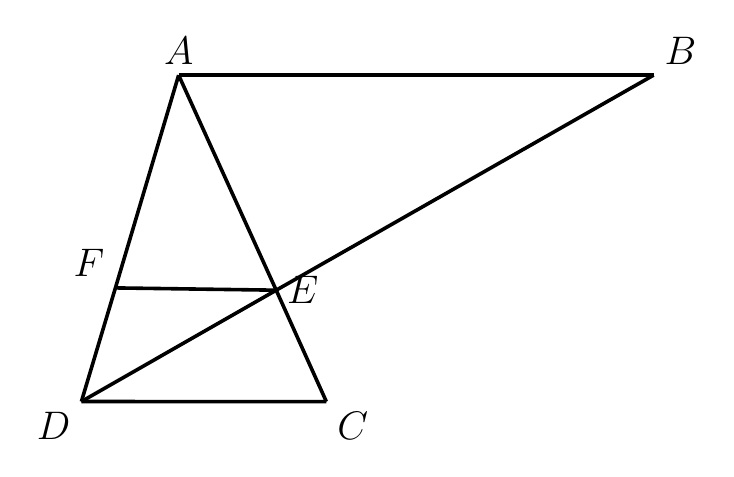
\begin{tikzpicture}[line width=1.3pt, line join=round]
\coordinate (A) at (-2.207,2.085);
\coordinate (B) at (3.825,2.085);
\coordinate (C) at (-0.331,-2.061);
\coordinate (D) at (-3.442,-2.060);
\coordinate (E) at (-0.968,-0.646);
\coordinate (F) at (-3.010,-0.617);









  
  \draw (A) -- (B);
  \draw (B) -- (E) -- (D);
  \draw (A) -- (E) -- (C);
  \draw (D) -- (C);
  \draw (A) -- (F) -- (D);
  \draw (F) -- (E);

  
  \node[above, font=\fontsize{13.5}{16.2}\selectfont] at (A) {$A$};
  \node[above right, font=\fontsize{13.5}{16.2}\selectfont] at (B) {$B$};
  \node[below right, font=\fontsize{13.5}{16.2}\selectfont] at (C) {$C$};
  \node[below left, font=\fontsize{13.5}{16.2}\selectfont] at (D) {$D$};
  \node[right, font=\fontsize{13.5}{16.2}\selectfont] at (E) {$E$};
  \node[above left, font=\fontsize{13.5}{16.2}\selectfont] at (F) {$F$};
\end{tikzpicture}
\end{document}